\section{Gestione del tempo tra quartieri}
Il problema principale della frammentazione della mappa in quartieri consiste nella gestione del $\Delta$ di avanzamento tra quartieri; i quartieri non possono avanzare indipendentemente l'uno dall'altro; cioè un quartiere che ha effettuato i calcoli per l'avanzamento per un certo $\Delta$, non può procedere a effettuare il calcolo di nuovi spostamenti per un nuovo $\Delta$ fino a quando tutti gli altri quartieri non hanno completato l'aggiornamento degli spostamenti delle entità al $\Delta$ precedente. Lo spostamento delle entità dei quartieri deve essere trasparente alla distribuzione della mappa, quindi un quartiere presenta una dipendenza dagli altri quartieri affinchè tutti i quartieri siano sincronizzati allo stesso quanto di tempo discretizzato. Ancora più evidente è il caso in cui un quartiere presenta un incrocio in cui per esempio una delle sue strade appartenga ad un altro quartiere; se il sistema non è sincronizzato allo stesso quanto di tempo si potrebbe incorrere nella situazione in cui un certo mezzo che debba essere spostato tra due quartieri, si trovi in attesa che il quartiere di destinazione si risincronizzi al quanto successivo; quindi avere una situazione in cui l'entità si trovi in attesa indipendentemente dalla velocità e dallo stato del traffico.\\
Dato che le entità attive del sistema sono le strade e gli incroci e la responsabilità dell'esecuzione del calcolo dell'avanzamento in un certo quanto di tempo è data sempre alle entità attive, queste dovranno essere partecipi nel regolamentare l'avanzamento del sistema al quanto di tempo successivo.\\

\subsection{Protocollo di sincronizzazione}
Questo protocollo si occupa di regolamentare l'avanzamento del sistema al quanto di tempo successivo; questo protocollo è quindi responsabile della gestione della logica di discretizzazione del tempo per permettere di avere una realtà continua consistente in ogni quartiere.\\
Per lo sviluppo di questo protocollo occorre considerare dapprima come il sistema viene avviato; cioè se il sistema attende che tutti i quartieri siano configurati e quindi tutti i quartieri partiranno in sincronia al tempo 0; oppure se si sceglie un approccio più flessibile in cui un quartiere viene configurato indipendentemente dagli altri e quindi entrerà in sincronizzazione in un momento non necessariamente corrispondente al tempo 0. Occorre considerare che un quartiere è una partizione a se stante, che presenta tuttavia delle dipendenze con gli altri quartieri; entrambi i sistemi di avvio presentano dei vantaggi: nel primo caso si ha che ogni quartiere aspetta che gli altri si siano configurati, si avrà quindi un ritardo nell'avvio, ma quando un quartiere ritorna dall'attesa può reperire ogni risorsa di qualunque altro quartiere dato che al ritorno dall'attesa il tutto è stato configurato; tuttavia seguendo questa idea si potrebbe presentare il caso in cui si potrebbero avere dei quartieri isolati che aspettano inutilmente altri quartieri o comunque si potrebbero voler aggiungere in seguito all'avvio della simulazione altri quartieri.\\
Il secondo caso invece è quello che si avvicina di più a ciò che è il paradigma della distribuzione, lasciando quindi l'indipendenza nella fase di avvio tra quartieri e quindi permettendo comunque lo spostamento di tutte le entità che presentano un percorso valido relativo al quartiere stesso, mentre per le entità che presentano delle destinazioni non raggiungibili il quartiere ne dovrà ritardare lo spostamento. Il nostro sistema implementa questa seconda scelta lasciando ove possibile l'indipendenza tra le partizioni permettendo l'avvio del sistema e quindi dello spostamento delle entità indipendentemente dal fatto che una partizione remota sia stata configurata o meno.\\
Solo quando un quartiere presenterà richiesta di sincronizzazione allora il sistema dovrà tener conto anche della sua richiesta per permettere l'avanzamento al quanto di tempo successivo in modo da coinvolgere ogni quartiere che necessita di essere sincronizzato.\\
Tuttavia se un quartiere è stato istanziato e ha iniziato l'operazione di sincronizzazione con gli altri quartieri, in caso di fallimento o di errore durante l'esecuzione di uno qualunque di questi quartieri sincronizzati il sistema non potrà che fermarsi dato che un quartiere esegue dei servizi di spostamento per conto di entità di altri quartieri; se un quartiere da errore durante l'esecuzione lo stato del sistema diviene inconsistente e occorre riavviare il sistema e se necessario farlo ripartire dall'ultima snapshot del sistema una volta istanziati tutti i quartieri che erano stati avviati e sincronizzati all'ultima snapshot disponibile.\\
Il protocollo di sincronizzazione dovrà quindi considerare la possibilità di accogliere dei nuovi quartieri da rendere parteci alla sincronizzazione.\\
Il protocollo di sincronizzazione si divide in due parti: la sincronizzazione tra entità attive del quartiere (\ref{int_synch}) e la sincronizzazione tra quartieri (\ref{quart_synch}).
\subsubsection{Sincronizzazione tra entità attive del quartiere}
\label{int_synch}
Ogni entità attiva del quartiere dovrà comunicare ad un gestore della sincronizzazione interna del quartiere, che ha eseguito l'aggiornamento dello stato di avanzamento delle entità passive per un certo $\Delta$ di sistema. L'entità attiva dovrà poi attendere che tutto il sistema sia sincronizzato con il $\Delta$ di sistema. Solo quando l'ultima entità attiva del quartiere in questione ha eseguito l'avanzamento al $\Delta$ di sistema allora questa entità potrà avviare il protocollo di sincronizzazione tra quartieri, vedi \ref{quart_synch}.

\subsubsection{Sincronizzazione tra quartieri}
\label{quart_synch}
Il seguente protocollo è un protocollo che esegue la sincronizzazione tra un numero di quartieri non fissato a priori. Di seguito i passi del protocollo (ogni volta che appare il nome di quartiere si intenderà l'entità responsabile della sincronizzazione di tutti i quartieri allocata nel quartiere stesso):
\begin{enumerate}
\item il quartiere deve ottenere dapprima dal name server il registro dei quartieri remoti che abbiano effettuato la registrazione della mappa al server gps (da notare che quartieri distinti potrebbero ricevere risposte diverse dal nameserver, ma risposte successive saranno sempre al più un sovrainsieme delle risposte date in precedenza);
\item il quartiere (Q\_X) per ogni quartiere presente nel registro dovrà inviare una notifica testimone del fatto che Q\_X è pronto per una nuova sincronizzazione. Tale notifica potrà essere eseguita dal quartiere interessato (Q\_Y) solo nel momento in cui anche Q\_Y è pronto per una nuova sincronizzazione, ovvero quando inizierà a eseguire anch'esso il protocollo (\ref{quart_synch}). L'esecuzione della procedura di notifica su Q\_Y andrà a buon fine nel caso in cui Q\_Y dispone nel proprio registro del quartiere Q\_X e in tal caso occorrerà salvare su Q\_Y il fatto che Q\_X è pronto per una nuova sincronizzazione; altrimenti Q\_Y accoda la notifica di Q\_X al fine di poterla gestire nel quanto successivo in cui a quel punto Q\_Y certamente otterrà dal name server anche Q\_X nello step 1 del protocollo. \\
Ogni quartiere ha degli eventi che permettono di decidere il momento in cui esso può eseguire le notifiche di richiesta di nuova sincronizzazione. L'evento che permette di eseguire le procedure di notifica su Q\_Y richieste da quartieri remoti Q\_X è il passaggio dall'esecuzione di \ref{int_synch} a \ref{quart_synch} e in particolare l'esecuzione dello step 1 del protocollo. \\ La disabilitazione dell'esecuzione della procedura di notifica su Q\_Y deve avvenire dall'ultimo quartiere utile che esegue su Q\_Y la procedura di notifica. Dove per ultimo quartiere utile si intende quell'ultimo quartiere (indipendentemente dall'ordine) che appartiene all'insieme minimo dei quartieri tra tutti gli insiemi di quartieri presenti nei registri dei quartieri stessi presi nello step 1 del protocollo (tale insieme d'ora in poi verrà chiamato \textit{MIN\_SET\_QUARTIERI}). \\
\item ogni quartiere presente in \textit{MIN\_SET\_QUARTIERI} dovrà quindi aspettare l'evento di chiusura della gestione delle notifiche di nuova sincronizzazione, d'ora in poi \textit{CLOSE\_SYNCH}; a questo punto un quartiere uscente dall'attesa non conosce più lo stato di avanzamento degli altri quartieri, cioè è solo a conoscenza del fatto che tutti i quartieri in \textit{MIN\_SET\_QUARTIERI} hanno presentato nuova richiesta di sincronizzazione, ma nel frattempo uno dei quartieri in \textit{MIN\_SET\_QUARTIERI} potrebbe aver iniziato nuovamente ad eseguire il protocollo sovrascrivendo l'esecuzione delle notifiche e quindi perdendo una notifica di nuova sincronizzazione da parte di un quartiere se l'evento \textit{CLOSE\_SYNCH} non era ancora giunto. Pertanto è necessario che ogni quartiere, prima di poter eseguire nuovamente una nuova sincronizzazione, attenda l'evento \textit{CLOSE\_SYNCH} che sarà inviato da ogni altro quartiere in \textit{MIN\_SET\_QUARTIERI};
\end{enumerate}
Tra lo step 1 e 2 occorre integrare il seguente punto:  
\begin{itemize}
\item il quartiere deve liberare dall'attesa, se presenti, tutti quei quartieri che al $\Delta$ di sincronizzazione precedente non erano nel registro dei quartieri, supponiamo che Q\_Y nel proprio registro non contenga Q\_X, mentre Q\_X contiene nel proprio registro Q\_Y; mentre il quartiere remoto Q\_X si presta in attesa sul quartiere Q\_Y, Q\_Y non considerà Q\_X. Quindi Q\_X deve essere classificato classificato come un quartiere nuovo che potrà entrare in sincronizzazione solo al $\Delta$ successivo; tuttavia Q\_X potrebbe nel frattempo già aver demandado l'esecuzione dello step 2 su altri quartieri che contenevano nel proprio registro Q\_X; ebbene questi quartieri dovranno ricordare tale fatto nel loro $\Delta$ di sincronizzazione successivo; mentre Q\_Y dovrà accodare Q\_X fino alla richiesta di sincronizzazione successiva in cui appunto verrà riaccodato dallo step appena descritto nella procedura di gestione delle notifiche per il nuovo $\Delta$.
\end{itemize}

\begin{figure}[H] % Example image
\center{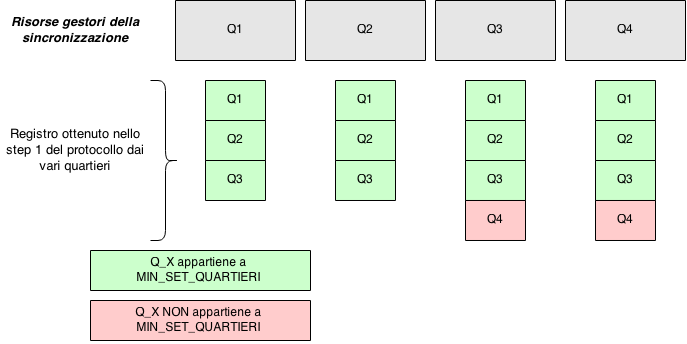
\includegraphics[width=1.0\linewidth]{ProtocolloSynch}}
\caption{Esempio di stato nella sincronizzazione dei quartieri.}
\label{fig:Esempio di stato nella sincronizzazione dei quartieri}
\end{figure}

Nell'esempio riportato i quartieri soggetti a sincronizzazione saranno Q1,Q2,Q3 mentre Q4 non potrà partecipare alla sincronizzazione, se non prima della sincronizzazione successiva in cui certamente Q1 e Q2 alla nuova richiesta del registro al name server otterranno anche Q4. Q4 cosa può fare dato che non può partecipare alla sincronizzazione? Esso potrebbe presentare una richiesta a Q1 o Q2 e in tal caso rimmarrebbe bloccato sul quartiere Q1 o Q2 dato che entrambi non dispongono di Q4; Q4 potrebbe anche presentare la richiesta a Q3 e in tal caso Q3 accoglierà Q4 e salverà temporaneamente una flag che lo avviserà per il prossimo quanto che Q4 ha già presentato richiesta di sincronizzazione. Q3 sa inoltre che non potrà attendere Q4 dato che nel momento in cui Q1 o Q2 presenteranno richiesta di sincronizzazione a Q3 invieranno anche il loro registro e li Q3 apprenderà che Q4 non è un quartiere sul quale occorre aspettare e quindi non è rilevante all'evento \textit{CLOSE\_SYNCH}. Con questo semplice esempio è stato presentato un caso di sincronizzazione; ma ce ne possono essere di più complicati per esempio nel caso in cui esistesse anche un quartiere Q5 non visibile a nessuno. In tal caso alla nuova sincronizzazione Q1 Q2 e Q3 memorizzeranno nel loro registro anche Q5, mentre per Q4 il quartiere Q5 sarà un quartiere nuovo e quindi potrà entrare in sincronizzazione solo al quanto successivo.

\paragraph{Considerazioni sul protocollo \ref{quart_synch}}
Questo protocollo si adatta dinamicamente a nuove richieste di sincronizzazione. Il difetto principale sta nel fatto che un quartiere dovrà attendere su altri quartieri al fine di apprendere se tutto il sistema è pronto per il passaggio al quanto successivo. In realtà l'attesa potrebbe essere rigirata sul quartiere stesso e non più sul quartiere remoto, ma data la limitazione sul numero massimo di quartieri non è un problema l'implementazione di questo protocollo anche se i quartieri utilizzano un thread-pool nella gestione delle richieste remote.